\documentclass[ifip]{svmult}
% choose options for [] as required from the list
% in the Reference Guide, Sect. 2.2
\usepackage{epsfig} 
\usepackage{makeidx}         % allows index generation
\usepackage{graphicx}        % standard LaTeX graphics tool
                             % when including figure files
\usepackage{multicol}        % used for the two-column index
\usepackage[bottom]{footmisc}% places footnotes at page bottom
% etc.
%\usepackage[demo]{graphicx}
\usepackage{subfig}
\usepackage{tabularx}
\usepackage{url}
\usepackage{ragged2e}
\usepackage{hyperref}
\usepackage{float}

\makeindex             % used for the subject index
                       % please use the style sprmidx.sty with
                       % your makeindex program
%%%%%%%%%%%%%%%%%%%%%%%%%%%%%%%%%%%%%%%%%%%%%%%%%%%%%%%%%%%%%%%%%%%%%

\begin{document}

%\title*{Analyzing FOSS Collaboration and Social Dynamics with Temporal Social Networks}
%\titlerunning{Analyzing FOSS Collab. \& Social Dynamics w/ Temporal Social Networks}
\title*{A Comparative Study of Developer Differences forks Versus Community-Driven Forks}
\titlerunning{Drawing the Big Picture: Temporal Visualization of Collaboration Graphs}

% Use \titlerunning{Short Title} for an abbreviated version of
% your contribution title if the original one is too long
%\author{Amir Azarbakht, Carlos Jensen}
\author{author name 1, author name 2}
% Use \authorrunning{Short Title} for an abbreviated version of
% your contribution title if the original one is too long
%\institute{Oregon State University, School of Electrical Engineering \& Computer Science\\ 1148 Kelley Engineering Center, Corvallis OR 97331, USA
\institute{university name\\ 
 address, country\\
%\texttt{\{azarbaam,cjensen\}@eecs.oregonstate.edu}}
%\texttt{http://eecs.oregonstate.edu/\textasciitilde azarbaam}}
%\texttt{http://eecs.oregonstate.edu/people/jensen}}
\texttt{\{author1,author2\}@department.university}\\
\texttt{http://department.university/\textasciitilde author1}\\
\texttt{http://department.university/\textasciitilde author2}}

%
% Use the package "url.sty" to avoid
% problems with special characters
% used in your e-mail or web address
%
\maketitle
\begin{abstract}
How can we understand FOSS collaboration better? Can social issues that emerge be identified and addressed as they happen? Can the community heal itself, become more transparent and inclusive, and promote diversity? We propose a technique to address these issues by quantitative analysis and temporal visualization of social dynamics in FOSS communities. We used social network analysis metrics to identify growth patterns and unhealthy dynamics; This gives the community a heads-up when they can still take action to ensure the sustainability of the project.\\
%\textbf{Keywords.} FOSS, Social Dynamics, Visualization, Temporal Visualization, Temporal Analysis, Free/Open Source Software, FLOSS, Forking, Social Network Analysis
\end{abstract}
\section{Introduction}
\label{sec:1}
% Always give a unique label
% and use \ref{<label>} for cross-references
% and \cite{<label>} for bibliographic references
% use \sectionmark{}
% to alter or adjust the section heading in the running head
Social networks are a ubiquitous part of our social lives, and the creation of online social communities has been a natural extension of this phenomena. Free/Open Source Software (FOSS) development efforts are prime examples of how community can be leveraged in software development, groups are formed around communities of interest, and depend on continued interest and involvement in order to stay alive [17].

Though the bulk of collaboration and communication in FOSS communities occurs online and is publicly accessible, there are many open questions about the social dynamics in FOSS communities. Projects might go through a metamorphosis when faced with an influx of new developers or the involvement of an outside organization. Conflicts between developers' divergent visions about the future of the project might lead to forking of the project and dilution of the community. Forking, either as a violent split when there is a conflict or as a friendly divide when new features are experimentally added both affect the community [3].

Most recent studies of FOSS communities have tended to suffer from an important limitation. They treat community as a static structure rather than a dynamic process. In this paper, we propose to use temporal social network analysis to study the evolution and social dynamics of FOSS communities. With these techniques we aim to identify measures associated with unhealthy group dynamics, e.g. a simmering conflict, as well as early indicators of major events in the lifespan of a community. One set of dynamics we are especially interested in, are those that lead FOSS projects to fork. We used the results of a study of forked FOSS projects by Robles and Gonzalez-Barahona [19] as the starting point for out study, and tried to gain a better understanding of the evolution of these communities.

This paper is organized as follows: We present related literature on online social communities. We then present the gap in the literature, and discuss why the issue needs to be addressed. After that, in methodology, we describe how gathering data, doing the analysis, and the visualization of the findings was carried out. At the end, we present results, discussion and threats to validity.
%\cite{monograph}.
\section{Related Work}
\label{sec:2}
% Always give a unique label
% and use \ref{<label>} for cross-references
% and \cite{<label>} for bibliographic references
% use \sectionmark{}
% to alter or adjust the section heading in the running head
The social structures of FOSS communities have been studied extensively. Researchers have studied the social structure and dynamics of team communications [4][10][11], identifying knowledge brokers and associated activities [20], project sustainability [10], forking [18] [19], their topology [4], their demographic diversity [13], gender differences in the process of joining them [12] and the role of the core team in their communities [21], etc. All of these studies have tended to look at community as a static structure rather than a dynamic process. This makes it hard to determine cause and effect, or the exact impact of social changes.

The study of communities has grown in popularity in part thanks to advances in social network analysis.  From the earliest works by Zachary [22] to the more recent works of Leskovec et al. [14][15], there is a growing body of quantitative research on online communities. The earliest works on communities was done with a focus on information diffusion in a community [22].  Zachary investigated the fission of a community, the process of communities splitting into two or more parts. He found that fission could be predicted by applying the Ford-Fulkerson min-cut algorithm [6] on the group's communication graph; ``the unequal flow of sentiments across the ties'' and discriminatory sharing of information lead to ``subcommunities with more internal stability than the community as a whole.'' 

Community splits in FOSS are referred to as forks, and are relatively common. Forking is defined as ``when a part of a development community (or a third party not related to the project) starts a completely independent line of development based on the source code basis of the project.'' Robles and Gonzalez-Barahona [19] identified 220 significant FOSS projects that have forked over the past 30 years, and compiled a comprehensive list of the dates and reasons for forking. They classified these into six main categories. (Table 3.) which we build on extensively. They identified a gap in the literature in case of ``how the community moves when a fork occurs''.

The dynamic behavior of a network and identifying key events was the aim of a study by Asur et al [1]. They studied three DBLP co-authorship networks and defined the evolution of these networks as following one of these paths: a) Continue, b) k-Merge, c) k-Split, d) Form, or e) Dissolve. They also defined four possible transformation events for individual members: 1) Appear, 2) Disappear, 3) Join, and 4) Leave. They compared groups extracted from consecutive snapshots, based on the size and overlap of every pair of groups. Then, they labeled groups with events, and used these identified events.
%
%\begin{table}
%\centering
%\caption{The measures of diversity used by [Asur
%et al. 2009]}
%\label{tab:1}       % Give a unique label
%%
%% For LaTeX tables use
%%
%\begin{tabular}{p{0.8in} p{3.8in}}
%\hline\noalign{\smallskip}
%\textbf{Metrics} & \textbf{Meaning} \\
%\noalign{\smallskip}\hline\noalign{\smallskip}
%Stability & Tendency of a node to have interactions with the same nodes over time \\ \hline
%Sociability & Tendency of a node to have different interactions \\\hline
%Influence & Number of followers a node has on a network and how its actions are copied and/or followed by other nodes. (e.g. when it joins/leaves a conversation, many other nodes join/leave the conversation, too) \\\hline
%Popularity & Number of nodes in a cluster (how crowded a sub-community is) \\
%\noalign{\smallskip}\hline
%\end{tabular}
%\end{table}
%
The communication patterns of FOSS developers in a bug repository were examined by Howison et al. [10]. They calculated out-degree centrality as their metric. Out-degree centrality measures the proportion of the number of times a node contacted other nodes (outgoing) over how many times it was contacted by other nodes (incoming). They calculated this centrality over time ``in 90-day windows, moving the window forward 30 days at a time.'' They found that ``while change at the center of FOSS projects is relatively uncommon,'' participation across the community is highly skewed, following a power-law distribution, where many participants appear for a short period of time, and a very small number of participants are at the center for long periods. Our approach is similar to theirs in how we form collaboration graphs and perform our temporal analysis. Our approach is different in terms of our project selection criteria, the metrics we examine, and our research questions.

The tension between diversity and homogeneity in a community was studied by Kunegis et al. [13]. They defined five network statistics used to examine the evolution of large-scale networks over time. They found that except for the diameter, all other measures of diversity shrunk as the networks matured over their lifespan. Kunegis et al. [13] argued that one possible reason could be that the community structure consolidates as projects mature.

%\begin{table}
%\centering
%\caption{The measures of diversity used by [Kunegis et al. 2012]}
%\label{tab:2}       % Give a unique label
%%
%% For LaTeX tables use
%%
%\begin{tabular}{p{1.3in}  p{1.8in}  p{1.7in}}
%\hline\noalign{\smallskip}
%\textbf{Network property} & \textbf{Network is diverse when} & \textbf{A network is diverse when} \\
%\noalign{\smallskip}\hline\noalign{\smallskip}
%Paths between nodes & Paths are long & Effective diameter \\ \hline
%Degrees of nodes  & Degrees are equal & Gini coefficient of the degree distribution \\ \hline
%Communities  & Communities have similar sizes & Fractional rank of the adjacency matrix \\ \hline
%Random walks  & Random walks have high probability of return & Weighted spectral distribution \\ \hline
%Control of nodes  & Nodes are hard to control & Number of driver nodes \\
%\noalign{\smallskip}\hline
%\end{tabular}
%\end{table}

Community dynamics was the focus of a recent study by Hannemann and Klamma [8] on three open source bioinformatics communities. They measured "age" of users, as starting from their first activity and found survival rates and two indicators for significant changes in the core of the community. They identified a survival rate pattern of 20-40-90\%, meaning that only 20\% of the newcomers survived after their first year, 40\% of the survivors survived through the second year, and 90\% of the remaining ones, survived over the next years. As for the change in the core, they suggested that a falling maximal betweenness in combination with an increasing network diameter as an indicator for a significant change in the core, e.g. retirement of a central person in the community. Our approach builds on top of their findings, and the evolution of betweenness centralities and network diameters for the projects in our study are depicted in the following sections.

To date, most studies on FOSS have only been carried out on a small number of projects, and using snapshots in time. To our knowledge, no study has been done of project forking that has taken into account the temporal dimension.

%\section{Motivation}
%\label{sec:3}
%% Always give a unique label
%% and use \ref{<label>} for cross-references
%% and \cite{<label>} for bibliographic references
%% use \sectionmark{}
%% to alter or adjust the section heading in the running head
%To better understand and measure the evolution and social dynamics of FOSS projects, integral components to understanding their evolution and direction, we need new and better tools. With this knowledge and these tools, we could help projects reflect on their actions, and help community leaders make informed decisions about possible changes or interventions. We want to map the dynamics of communities to real world phenomena. Identification is the first step to rectify an undesired dynamic before the damage is done. A community that does not manage growing pains may end up stagnating or dissolving. 
%
%Managing growing pains is especially important in case of FOSS, where near half the project contributors are volunteers [Forrest et al. 2012]. [Oh et al. 2004] have argued that openness in FOSS is ``[...] generally perceived as having a positive connotation, however, the term can also be interpreted as referring to some unconstructive characteristics, such as unobstructed exit, susceptible, vulnerable, fragile, lacking effective regulation, and so on. The unobstructed exit and lack of regulatory force inherent in the OSS community can result in a community's susceptibility and vulnerability to herded exits by its participants. Commercial vendor intervention, an alternative project becoming available, and licensing issues can result in some original core members ceasing to provide their loyal service for the community, which can prompt their coworkers to leave as well'' [Oh et al. 2004].
%
%Recipes for success or stagnation, sustainability or fragmentation could be identifiable, leading to a set of best practices and pitfalls. 

%\section{Research Questions}
%\label{sec:4}
% Always give a unique label
% and use \ref{<label>} for cross-references
% and \cite{<label>} for bibliographic references
% use \sectionmark{}
% to alter or adjust the section heading in the running head
%We argue that the social interactions data reflects the changes the community goes through, and will be able to describe the context surrounding a forking event. Robles and Gonzalez-Barahona [Robles and Gonzalez-Barahona 2012] classify the main reasons for forking into six classes, listed in Table 3.
%
%\begin{table}
%\centering
%\caption{The main reasons for forking as classified by [Robles and Gonzalez-Barahona 2012]}
%\label{tab:3}       % Give a unique label
%%
%% For LaTeX tables use
%%
%\begin{tabular}{p{2.5in} p{1.8in}}
%\hline\noalign{\smallskip}
%\textbf{Reason for forking} & \textbf{Example forks} \\
%\noalign{\smallskip}\hline\noalign{\smallskip}
%Technical (Addition of functionality) & Amarok \& Clementine Player \\ \hline
%More community-driven development & Asterisk \& Callweaver \\ \hline
%Discontinuation of the original project & Apache web server \\ \hline
%Commercial strategy forks & LibreOffice \& OpenOffice.org \\ \hline
%Legal issues & X.Org \& XFree \\ \hline
%Differences among developer team & Kamailio \& OpenSIPS \\ 
%\noalign{\smallskip}\hline
%\end{tabular}
%\end{table}
%
%Three of the six listed reasons are socially related, and so should arguably be reflected somehow in the social interaction data. As an example, if a fork occurs because of a desire for ``more community-driven development'', we expect to see an interaction patterns in the collaboration data showing a strongly-connected core that is hard to penetrate for the rest of the community. In other words, the power stays in the hands of the same people throughout, as new people come and go.
%
%We aimed to visualize and quantify how the community is structured, how it evolves, and the degree to which community involvement changes over time. To this end we adopted a methodology that is described in the next section.

%\subsubsection{Hypothesis \#1:}
%Social interactions data can be used to predict an imminent fork. 
%
%\subsubsection{Hypothesis \#2:}
%\textit{``Personal differences''} and \textit{``technical differences''} are associated with distinctly different interaction patterns. It is possible to tell the difference between when the reason for forking was personal vs. technical. 
%
%\subsubsection{Hypothesis \#3:}
%It is possible to tell through collaboration patterns between when the reason for forking is \textit{``more community-driven development''} and \textit{``differences among the developer team''}.

\section{Methodology}
\label{sec:5}

We argue that the social interactions data reflects the changes the community goes through, and will be able to describe the context surrounding a forking event. Robles and Gonzalez-Barahona [19] classify forking into six classes, listed in Table 1, based on the motives for forking.

\begin{table}
\centering
\caption{The main reasons for forking as classified by Robles and Gonzalez-Barahona [19]}
\label{tab:3}       % Give a unique label
%
% For LaTeX tables use
%
\begin{tabular}{p{2.5in} p{1.8in}}
\hline\noalign{\smallskip}
\textbf{Reason for forking} & \textbf{Example forks} \\
\noalign{\smallskip}\hline\noalign{\smallskip}
Technical (Addition of functionality) & Amarok \& Clementine Player \\ \hline
More community-driven development & Asterisk \& Callweaver \\ \hline
Differences among developer team & Kamailio \& OpenSIPS \\ \hline
Discontinuation of the original project & Apache web server \\ \hline
Commercial strategy forks & LibreOffice \& OpenOffice.org \\ \hline
Legal issues & X.Org \& XFree \\
\noalign{\smallskip}\hline
\end{tabular}
\end{table}

The first three of the six motives listed are social, and so should arguably be reflected in the social interaction data. For example, if a fork occurs because of a desire for ``more community-driven development'', we would perhaps expect to see patterns in the data showing a strongly-connected core that is hard to penetrate for the rest of the community prior to the fork. In other words, the power stays in the hands of the same people over a long period of time while new people come and go. Our goal was to visualize and quantify how the community is structured, how it evolves, and the degree to which involvement changes over time. To this end, we picked projects from the aforementioned three categories of forked projects. This involved obtaining communication archives, creating the collaboration graphs, applying social network analysis (SNA) techniques to measure key metrics, and visualizing the evolving graphs. We did this in four phases as described in the following:

\subsection{Phase 1: Data Collection}
	 
The study of forks by Robles and Gonzalez-Barahona [19] included information on 220 forks and their reasons. We applied three selection criteria to those projects. A project was short-listed if it was recent, i.e. the fork had happened after the year 2000; data was available; and their communities were of approximately the same size. This three stage filtering process resulted in the projects listed in Table 2. 

\begin{table}
\centering
\caption{Forked projects for which collaboration data was collected}
\label{tab:3}       % Give a unique label
%
% For LaTeX tables use
%
\begin{tabular}{p{1.8in} p{2.3in} p{0.5in}}
\hline\noalign{\smallskip}
\textbf{Projects} & \textbf{Reason for forking} & \textbf{Year} \\
\noalign{\smallskip}\hline\noalign{\smallskip}
Amarok \& Clementine Player & Technical (Addition of functionality) & 2010\\ \hline
Asterisk \& Callweaver & More community-driven development & 2007\\ \hline
Kamailio \& OpenSIPS & Differences among developer team & 2008 \\ 
\noalign{\smallskip}\hline
\end{tabular}
\end{table}
Data collection involved analyzing mailing list archives. We collected data for the year in which the fork happened, as well as for three month before and three months after that year in order to capture the social context context at the time of the fork.

\subsection{Phase 2: Creating Communication Graphs}

Many social structures can be represented as graphs. The nodes represent actors/players and the edges represent the interaction between them. Such graphs can be a snapshot of a network -- a static graph -- or a changing network, also called a dynamic graph. In this phase, we processed the data to form a communication graph of the community. We were looking for how people interacted with each other. We decided to treat the general mailing list as a person, because the bulk of the communication was targeted at it, and most newcomers start by sending their questions to the general mailing list. Each communication effort was captured with a time-stamp. This allowed us to form a dynamic graph, in which the nodes would exist if and only if they had an interaction with another node during the period we were interested in.

\subsection{Phase 3: Temporal Visualization and Temporal Evolution Analysis }

In this phase, we wanted to analyze the changes that happen to the community over a given period of time, i.e. three months before and three months after the year in which the forking event happened. We measured betweenness centrality [5] of the most significant nodes in the graph, and the graph diameter over time. Figures 2-4 show the betweenness centralities over the 1.5 year period for the Camailio, Amarok and Asterisk projects respectively. To do temporal analysis, we had two options; 1) look at snapshots of the network state over time, (e.g. to look at the network snapshots in every week, the same way that a video is composed of many consecutive frames), and 2) look at a period through a time window. We preferred the second approach, and looked through a time window of three months wide with 1.5 month overlaps. To create the visualizations, we used a 3 months time frame that progressed six days a frame. In this way, we had a relatively smooth transition.
%There are many ways of looking at an individual's importance. One is called \textit{closeness centrality}. The \textit{farness} of a node is defined as the sum of its distances to all other nodes. The \textit{closeness} of a node is defined as the inverse of the farness. More informally, the more central a node is the lower its total distance to all other nodes. \textit{Closeness centrality} can be used as a measure of how fast information will spread through the network [Chakrabarty and Faloutsos 2006]. Secondly, if we are looking for people who can serve as bridges between two distinct communities, we could measure the node's \textit{betweenness centrality}. Betweenness centralities for mediators who act as intermediate entities between other nodes are higher [Chakrabarty and Faloutsos 2006].  Third, if cross-community collaboration is the focus, we can measure \textit{edge betweenness centrality}.  Edges connecting nodes from different communities have higher edge centrality values. In the community collaboration graph, edge betweenness or stress of an edge is the number of these shortest paths that the edge belongs to, considering all shortest paths between all pairs of nodes in the graph. Fourth, one can claim that certain people in the community are more important than others, and whoever is close to them, is relatively more important than others. In graph terms, this is measured by \textit{eigenvector centrality}, which is based on the assumption that connections to high-profile nodes contribute more to the importance of a node. Google's PageRank link-analysis algorithm by [Brin and Page 1998] is a variant of the eigenvector centrality measure. In short, centrality measures have been used in several studies to identify key player in a community.

%\begin{figure}[!htbp]
%\centering
%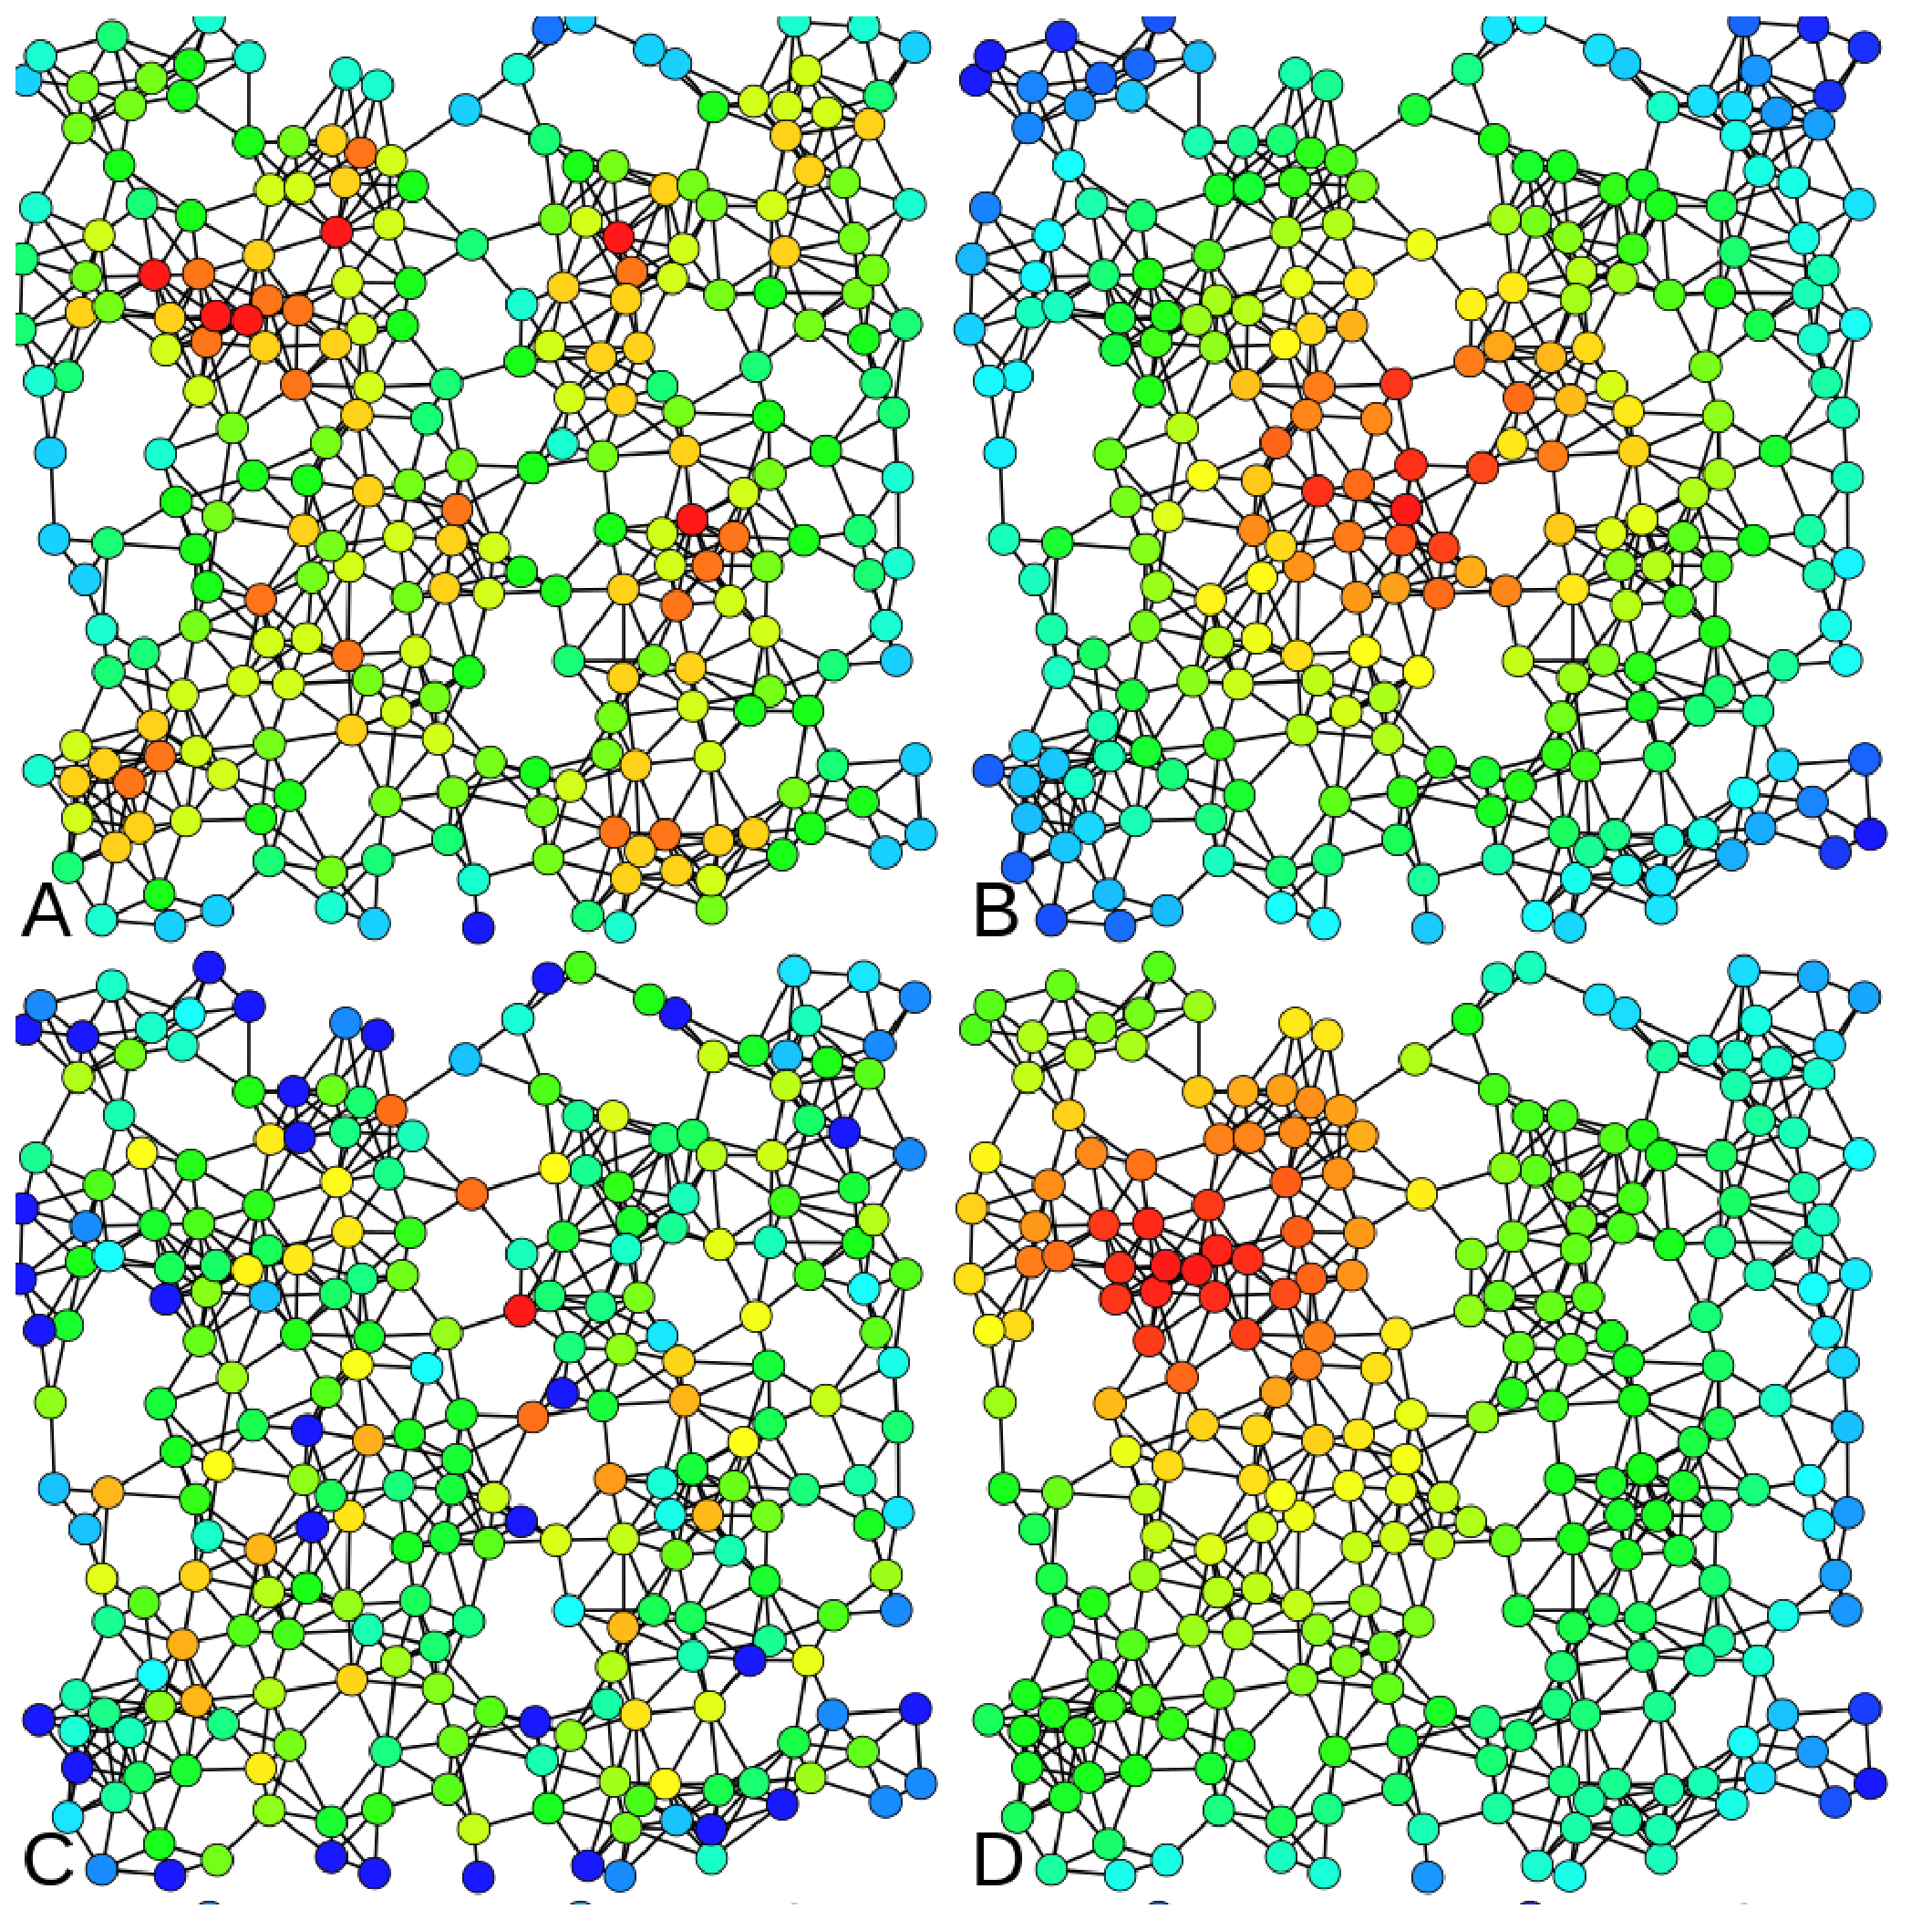
\epsfig{file=centrality.eps, width=3.33in}
%\caption{Heat-map color-coded examples of nodes with high centrality metric are shown above. The same network is analysed four times with the following centrality measures:  A) Degree centrality, B) Closeness centrality, C) Betweenness centrality and D) Eigenvector centrality [Rocchini 2012]}
%\end{figure}
%
%In addition to the centrality measures, we planned to look into the \textit{resilience} of the community as well. By resilience, we mean how well the network holds its structure and form when some parts of it are deleted, added, or changed. For a graph, the resilience of a graph is a measure of its robustness to node or edge failures. This could occur for instance when an influential member of the community leaves. Many real-world graphs are resilient to random failures but vulnerable to targeted attacks. Resilience can be related to the \textit{graph diameter}: a graph whose diameter does not increase much on node or edge removal has higher resilience [Chakrabarty and Faloutsos 2006].
%\subsection{Phase 4: Temporal Visualization}
%Several visualization techniques and tools are used in the field of social network analysis, for instance, NetLogo [Wilensky 1999], igraph [Csardi and Nepusz 2006], NetworkX [Hagberg et al. 2008], SoNIA [Bender-deMoll and McFarland 2006], NodeXL [Smith et al. 2009]. Gephi, is a FLOSS tool for exploring and manipulating networks. It is capable of handling large networks with more than 20,000 nodes and features several SNA algorithms. It is customizable with plugins and we used it for dynamic network visualization.
We visualized the dynamic network changes using Gephi [2]. The videos show how the community graph is structured, using a continuous force-directed linear-linear model, in which the nodes are positioned near or far from each other proportional to the graph distance between them. This results in a graph shape between between Fr\"{u}chterman \& Rheingold's [7] layout and Noack's LinLog [16].

\section{Results and Discussion}
\label{sec:6}
% Always give a unique label
% and use \ref{<label>} for cross-references
% and \cite{<label>} for bibliographic references
% use \sectionmark{}
% to alter or adjust the section heading in the running head
\subsection{Kamailio Project}
Figure 1 shows four key frames from the Kamailio project's social graph around the time of their fork (the events described here are easier to fully grasp by watching the video. A node's size in a proportional to the number of interactions the node (contributor) has had within the study period and the position and edges of the nodes change if they had interactions within the time window shown, with six day steps per frame. The 1 minute and 37 seconds video shows the life of the Kamailio project between October 2007, and March 2009. Nodes are colored based on the modularity of the network. 

The community starts with the GeneralList as the the biggest node, and four larger core contributors and three lesser size core contributors. The big red-colored node's transitions are hard to miss, as this major contributor departs from the core to the periphery of the network (Video minute 1:02) and then leaves the community (Video minute 1:24) capturing either a conflict or retirement. This corresponds to the personal difference category of forking reasons.
\begin{figure} 
\def\tabularxcolumn#1{m{#1}} 
\begin{tabularx}{\linewidth}{@{}cXX@{}}
\begin{tabular}{cccc} 
\subfloat[]{\includegraphics[width=3cm,height=3cm]{2}} 
&
\subfloat[]{\includegraphics[width=3cm,height=3cm]{3}}
&
\subfloat[]{\includegraphics[width=3cm,height=3cm]{5}} 
& 
\subfloat[]{\includegraphics[width=3cm,height=3cm]{7}}
\end{tabular} 
\end{tabularx} 
\caption{Snapshots from video visualization of Kamailio's graph (Oct. 2007 - Mar. 2009) in which a core contributor (colored red) moves to the periphery and eventually departs the community.} 
\label{foo} 
\end{figure} 

\begin{figure}[!htbp]
\centering
\epsfig{file=Kamailio_chart.eps, width=5in}
\justifying
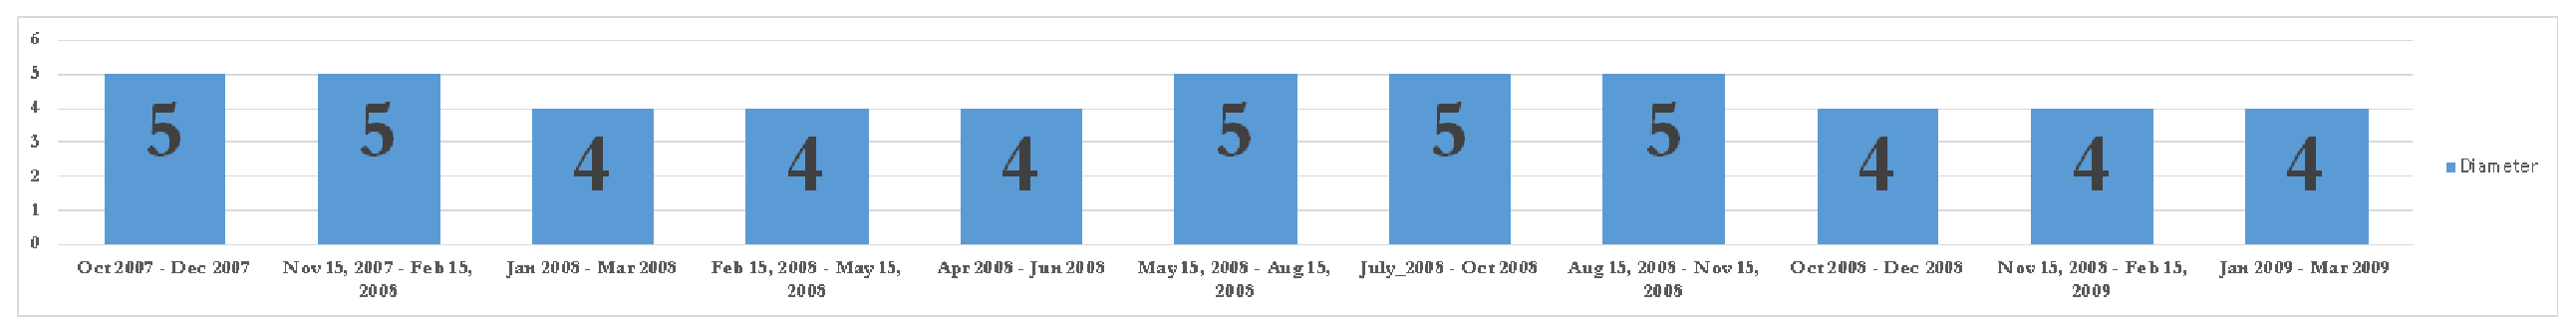
\epsfig{file=Kamailio_diameter.eps, width=4.523in}
\caption{Kamailio top contributors' betweenness centralities and network diameter over time (Oct. 2007 to Mar. 2009) in 3-month time windows with 1.5-month overlaps}
\end{figure}

%\begin{figure}[!htbp]
%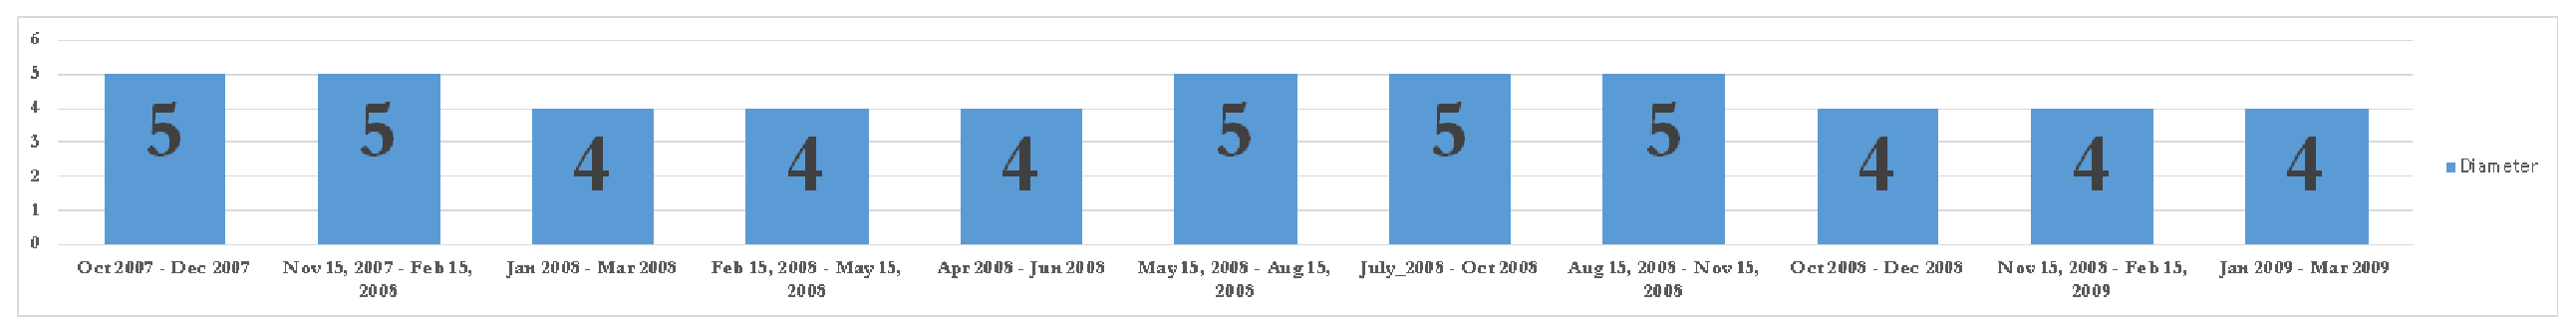
\epsfig{file=Kamailio_diameter.eps, width=4.6in}
%\caption{Kamailio project's diameter over time between October 2009 to March 2011 in 3-months time windows with 1.5 months overlaps}
%\end{figure}

Figure 2 shows the betweenness centrality of the major contributors of Kamailio project over the same time period. The horizontal axis marks the dates, (each mark represents a 3-month time window with 1.5 months overlap). The vertical axis shows the percentage of the top betweenness centralities for each node. The saliency of the GeneralList -- colored as light blue -- is apparent due to to its continuous and dominant presence in the stacked area chart. The chart legend lists the contributors based on the color and in the same order of appearance on the chart starting from the bottom. One can easily see that around the "Aug. 15, 2008 - Nov. 15, 2008" tick mark on the horizontal axis, several contributors' betweenness centralities shrink to almost zero and disappear. This helps identify the date of fork with a month accuracy. The network diameter of the Kamailio project over the same time period is also shown in Figure 3. The increase in the network diameter during this period confirms the findings of Hannemann and Klamma [8]. 

This technique can be used to identify the people involved in conflict and the date the fork happened with a months accuracy, even if the rival project does not emerge immediately.
\subsection{Amarok Project}
The video for the Amarok project fork is available online\footnote{Video visualizations available at \href{http://eecs.oregonstate.edu/~azarbaam/OSS2014/}{http://eecs.oregonstate.edu/\textasciitilde azarbaam/OSS2014/}}, and the results from our quantitative analysis of the betweenness centralities and the network diameters are shown in Figure 3. The results show that the network diameter has not increased over the period of the fork, which shows a resilient network. The video shows the dynamic changes in the network structure, again typical of a healthy network, rather than of simmering conflict. These indicators show that Amarok fork in 2010 arguably belongs to the ``addition of technical functionality'' rationale for forking, as there are no visible social conflict. 

\begin{figure}[!Htbp]
\centering
\epsfig{file=Amarok_chart.eps, width=5in}
\justifying
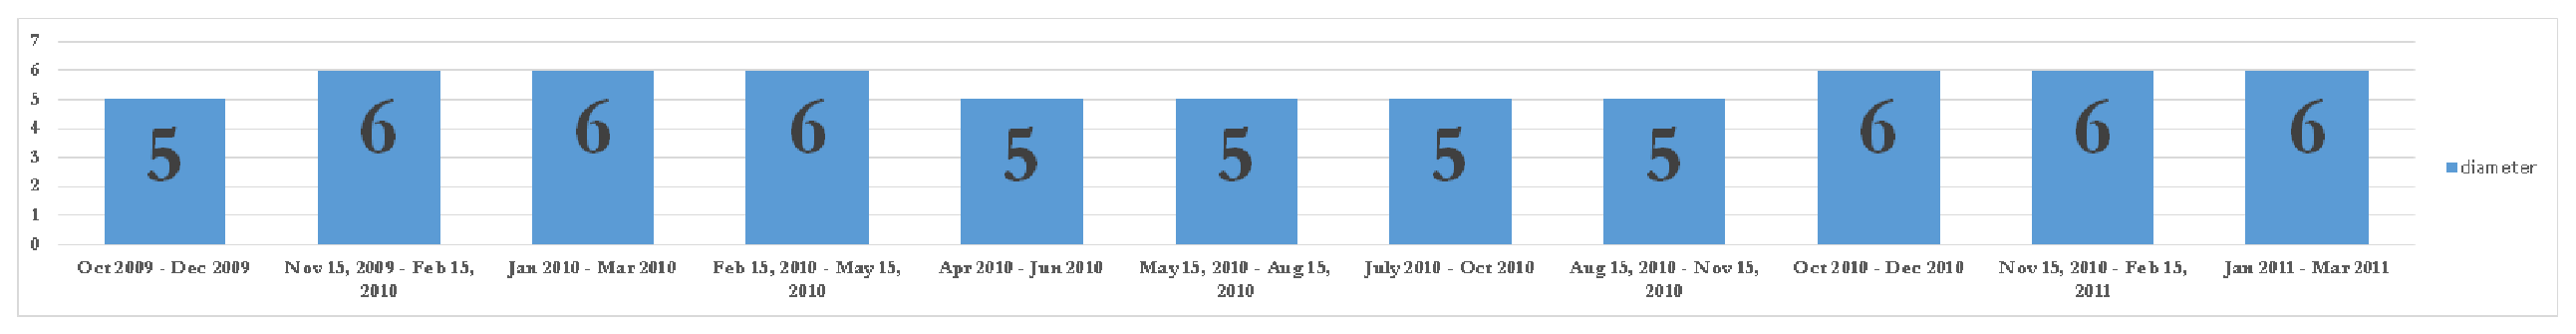
\epsfig{file=Amarok_diameter.eps, width=4.62in}
\caption{Amarok project's top contributors' betweenness centralities and network diameter over time between Oct. 2009 to Mar. 2011 in 3-months time windows with 1.5 months overlaps}
\end{figure}

\subsection{Asterisk Project}
The video for the Asterisk project is also available online, and the results from our quantitative analysis of the betweenness centralities and the network diameters are shown in Figure 4. The results show that the network diameter remained steady at 6 throughout the period. The Asterisk community was by far the most crowded project, with 932 nodes and 4282 edges. The stacked area chart shows the distribution of centralities, where we see an 80\%-20\% distribution (, i.e. 80\% or more of the activity is attributed to six major players, with the rest of the community accounting for only 20\%). This is evident in the video representation as well, as the top-level structure of the network holds throughout the time period. The results from the visual and quantitative analysis links the Asterisk fork to the more community-driven category of forking reasons.

\begin{figure}[!Htbp]
\label{Asterisk_chart}
\centering
\epsfig{file=Asterisk_chart.eps, width=5in}
\justifying
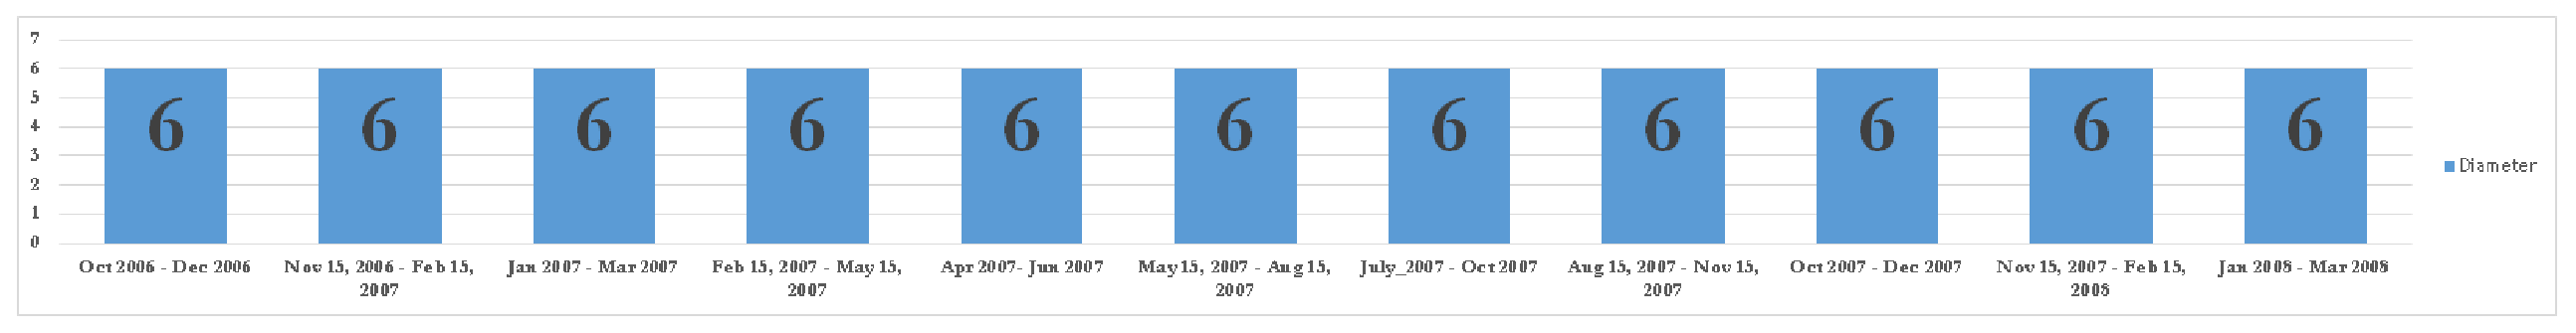
\epsfig{file=Asterisk_diameter.eps, width=4.67in}
\caption{Asterisk project's top contributors' betweenness centralities and network diameter over time between Oct. 2009 to Mar. 2011 in 3-months time windows with 1.5 months overlaps}
\end{figure}
\section{Conclusion}
We studied the collaboration networks of three FOSS projects using a combination of temporal visualization and quantitative analysis. We based our study on two papers by Robles and Gonzalez-Barahona [19] and Hannemann and Klamma [8], and identified three projects that had forked in the recent past. We mined the collaboration data, formed dynamic collaboration graphs, and measured social network analysis metrics over an 18-month period time window. 

We also visualized the dynamic graph (available online) and as stacked area charts over time. The visualizations and the quantitative results showed the differences among the projects in the three forking reasons of personal differences among the developer teams, technical differences (addition of new functionality) and more community-driven development. The personal differences representative project was identifiable, and so was the date it forked, with a month accuracy. The novelty of the approach was in applying the temporal analysis rather than static analysis, and in the temporal visualization of community structure. We showed that this approach shed light on the structure of these projects and reveal information that cannot be seen otherwise.
%\section{Threats to Validity}
%The presented findings may not be generalized to all OSS projects. The projects studies in this paper were selected from a pool of candidate projects, partly because data about them was available. Given access, a better sampling approach has to be adopted, which could result in a more robust investigation. Furthermore, the proposed technique uses the data from online communications. The assumption that all the communication can be captured by mining repositories is intuitively imperfect, but inevitable. Hence, to minimize the effect of this assumption, we plan to complement the quantitative approach with a qualitative approach of interviewing key individuals from the community as future work.
%\section{Future Work}
%Considering the novelty of temporal dynamic analysis and temporal visualization, there is ample possibility for further studies. To validate the results of this study, the proposed technique could be applied to other OSS project forks, with additional parameters. In today's world of big data, the possibilities are numerous for formulating novel well-formed research questions. 

%%%%%%%%%%%%%%%%%%%%%%%%%%%%%%%%%%%%%%%%%%%%%%%%%%%%%%%%%%%%%%%%%%%%%%%%%%

\begin{table}
\centering
\caption{Projects forked because of personal difference among the developer team, found as Robles and Gonzalez-Barahona [19] sorted in chronological order, and their data availability}
\label{tab:3}       % Give a unique label
\begin{tabular}{p{0.92in} p{0.8in} p{0.8in} p{1.7in} p{0.6in}}
\hline\noalign{\smallskip}
\textbf{Original} & \textbf{Forked} & \textbf{Date} & \textbf{Data available?} & \textbf{Collected?}\\
\noalign{\smallskip}\hline\noalign{\smallskip}
GNU Emacs & X Emacs & 1991, ? & No, Only after Sept 2000 & N/A \\ \hline
NetBSD & OpenBSD & 1995, Oct & Yes, but scarce & N/A \\ \hline
xMule & aMule & 2003, Aug & No, only 2006-2007 & N/A \\ \hline
lMule & xMule & 2003, Jun & No & N/A \\ \hline
Sodipodi & Inkscape & 2003, Nov & Yes & Req.\\ \hline
Nucleus CMS & Blog:CMS & 2004, May & No, only after Sept 2004 & N/A \\ \hline
BMP & Audacious & 2005, Oct & Yes & Req. \\ \hline
ntfsprogs & NTFS-3G & 2006, Jul & No & N/A \\ \hline
OpenWRT & FreeWRT & 2006, May & No, only after Oct 2006 & N/A \\ \hline
QtiPlot & SciDavis & 2007, Aug & No & N/A \\ \hline
\textbf{Kamailio} & OpenSIPS & 2008, Aug & Yes & \textbf{Yes} \\ \hline
Blastwave.org & OpenCSW & 2008, Aug & No & N/A \\ \hline
jMonkeyEngine & Ardor3D & 2008, Sept & but scarce & N/A \\ \hline
Frog CMS & Wolf CMS & 2009, Jul & No & N/A \\ \hline
Aldrin & Neil & 2009, ? & No & N/A \\ \hline
\textbf{Ffmpeg} & libav & 2011, Mar & Yes & \textbf{Yes}\\
\noalign{\smallskip}\hline
\end{tabular}
\end{table}


%%%%%%%%%%%%%%%%%%%%%%%%%%%%%%%%%%%%%%%%%%%%%%%%%%%%%%%%%%%%%%%%%%%%%%%%%%%%%%%%
\begin{table}
\centering
\caption{Projects forked because of the need for more community-driven development by Robles and Gonzalez-Barahona [19] sorted in chronological order}
\label{tab:4}
\begin{tabular}{p{0.95in} p{0.85in} p{0.7in} p{1.4in} p{0.4in}}\hline\noalign{\smallskip}
\textbf{Original} & \textbf{Forked} & \textbf{Date} & \textbf{Data available?} & \textbf{Collected?}\\
\noalign{\smallskip}\hline\noalign{\smallskip}
Nethack & Slash'EM & 1996, ? & No & N/A \\ \hline
GCC & EGCS & 1997, ? & No & N/A \\ \hline
SourceForge & Savane & 2001, Oct & No & N/A \\ \hline
PHPNuke & PostNuke & 2001, Sum & Not found & N/A \\ \hline
QTExtended & OPIE & 2002, May & No & N/A \\ \hline
GraphicsMagick & Graphics & 2002, Nov  & No, only after 2003 & N/A \\ \hline
\textbf{freeglut} & OpenGLUT & 2004, Mar & Yes & \textbf{Yes} \\ \hline
Mambo & Joomla! & 2005, Aug & No & N/A \\ \hline
SER & Kamailio & 2005, Jun & No, only after 2006 & N/A \\ \hline
PHPNuke & RavenNuke & 2005, Nov & Not found & N/A \\ \hline
Hula & Bongo & 2006, Dec & No & N/A \\ \hline
Compiere & A Dempiere & 2006, Sept & No dev mailing list & N/A \\ \hline
Compiz & Beryl & 2006, Sept & No, only after Jun 2007 & N/A \\ \hline
SQL-Ledger & LedgerSMB & 2006, Sept & No dev mailing list & N/A \\ \hline
\textbf{Asterisk} & Callweaver & 2007, Jun & Yes & \textbf{Yes} \\ \hline
CodeIgniter & KohanaPHP & 2007, May & Not found & N/A \\ \hline
OpenOffice.org & Go-oo.org & 2007, Oct & No, only after Jun 2011 & N/A \\ \hline
Mambo & MiaCMS & 2008, May & No & N/A \\ \hline
TORCS & Speed Dreams & 2008, Nov & Yes, but scarce & N/A \\ \hline
MySQL & MariaDB & 2009, Jan & Yes & No\\ \hline
Nagios & Icinga & 2009, May & Yes & Req \\ \hline
Project Darkstar& RedDwarf & 2010, Feb & Yes, but scarce & N/A \\ \hline
SysCP & Froxlor & 2010, Feb & N/A & N/A \\ \hline
Dokeos & Chamilo & 2010, Jan & Not found & N/A \\ \hline
GNU Zebra & Quagga & 2010, Jul & No & N/A \\ \hline
\textbf{rdesktop} & FreeRDP & 2010, Mar & Yes & \textbf{Yes} \\ \hline
OpenOffice.org & LibreOffice & 2010, Sept & No, only after Jun 2011 & N/A \\ \hline
Redmine & ChiliProject & 2011, Feb & Yes, but scarce & N/A \\
\noalign{\smallskip}\hline
\end{tabular}
\end{table}


%\section*{Acknowledgements}
%\label{sec:7}
%% Always give a unique label
%% and use \ref{<label>} for cross-references
%% and \cite{<label>} for bibliographic references
%% use \sectionmark{}
%% to alter or adjust the section heading in the running head
%We would like to thank the Amarok, Asterisk and Kamailio project members for making their data available, without which this study would not have been possible. 

% BibTeX users please use
% \bibliographystyle{}
% \bibliography{}
%
% Non-BibTeX users please follow the syntax
% the syntax of "referenc.tex" for your own citations
%%%%%%%%%%%%%%%%%%%%%%%% referenc.tex %%%%%%%%%%%%%%%%%%%%%%%%%%%%%%
% sample references
% "computer science"
%
% Use this file as a template for your own input.
%
%%%%%%%%%%%%%%%%%%%%%%%% Springer-Verlag %%%%%%%%%%%%%%%%%%%%%%%%%%
%
% BibTeX users please use
% \bibliographystyle{}
% \bibliography{}
%
% Non-BibTeX users please use
\begin{thebibliography}{99.}
%
% and use \bibitem to create references.
%
% Use the following syntax and markup for your references
%
%% Monographs
%\bibitem{monograph} Kajan E (2002)
%Information technology encyclopedia and acronyms. Springer, Berlin
%Heidelberg New York
%
%% Contributed Works
%\bibitem{contribution} Broy M (2002) Software engineering -- From
%auxiliary to key technologies. In: Broy M, Denert E (eds)
%Software Pioneers. Springer, Berlin Heidelberg New York
%
%% Journal
%\bibitem{journal} Che M, Grellmann W, Seidler S (1997)
%Appl Polym Sci 64:1079--1090
%
%\bibitem{journal} Chde M, Grellmann W, Seidler S (1997)
%Appl Polym Sci 64:1079--1090
%
%%% Theses
%%\bibitem{thesis} Ross DW (1977) Lysosomes and storage diseases. MA
%%Thesis, Columbia University, New York
%
\bibitem{Asur} Asur, S., S. Parthasarathy, and D. Ucar, (2009), ``\textit{An event-based framework for characterizing the evolutionary behavior of interaction graphs,}'' ACM Trans.  Knowledge Discovery Data. 3, 4, Article 16, (November 2009), 36 pages. 2009.

\bibitem{AzarbakhtOSS2014} Azarbakht, A. and C. Jensen, ``\textit{Drawing the Big Picture: Temporal Visualization of Dynamic Collaboration Graphs of OSS Software Forks,}'' Proc. 10th Int'l. Conf. Open Source Systems, 2014.

\bibitem{AzarbakhtINSNA2014} Azarbakht, A. and C. Jensen, ``\textit{Temporal Visualization of Dynamic Collaboration Graphs of OSS Software Forks,}'' Proc. Int'l. Network for Social Network Analysis (INSNA) Sunbelt XXXIV Conf., 2014.

\bibitem{AzarbakhtOpenSym2013} Azarbakht, A., ``\textit{Drawing the Big Picture: Analyzing FLOSS Collaboration with Temporal Social Network Analysis,}'' Proc. 9th Int'l. Symp. Open Collaboration, ACM, 2013.

\bibitem{AzarbakhtOSS2013} Azarbakht, A. and C. Jensen, ``\textit{Analyzing FOSS Collaboration \& Social Dynamics with Temporal Social Networks,}'' Proc. 9th Int'l. Conf. Open Source Systems Doct. Cons., 2013.

\bibitem{AzarbakhtVLHCC2014} Azarbakht, A., ``\textit{Temporal Visualization of Collaborative Software Development in FOSS Forks,}'' Proc. IEEE Symp. Visual Languages and Human-Centric Computing, 2014.

\bibitem{Baishakhi} Baishakhi R., C. Wiley, and M. Kim, ``\textit{REPERTOIRE: a cross-system porting analysis tool for forked software projects,}'' Proc. ACM SIGSOFT 20th Int'l. Symp. Foundations of Software Engineering, ACM, 2012.

\bibitem{Bastian} Bastian, M., S. Heymann, and M. Jacomy, ``\textit{Gephi: an open source software for exploring and manipulating networks,}'' Int'l AAAI Conf. on Weblogs and Social Media, 2009.

\bibitem{Bezrukova} Bezrukova, K,, C. S. Spell, J. L. Perry, ``\textit{Violent Splits Or Healthy Divides? Coping With Injustice Through Faultlines,}'' Personnel Psychology, Vol 63, Issue 3. 2010. 

\bibitem{Bird} Bird, C., D. Pattison, R. D'Souza, V. Filkov, and P. Devanbu, ``\textit{Latent social structure in open source projects,}'' Proc. 16th ACM SIGSOFT Int'l. Symposium on Foundations of software engineering, ACM, 2008.  

\bibitem{Brandes} Brandes, U. ``\textit{A Faster Algorithm for Betweenness Centrality}'', Journal of Mathematical Sociology 25(2):163-177, 2001.

\bibitem{Chakrabarti} Chakrabarti,  D., and C. Faloutsos. ``\textit{Graph mining: Laws, generators, and algorithms,}'' ACM Computing Surveys, 38, 1, Article 2, 2006.

\bibitem{Coleman1964} Coleman, J.S. ``\textit{Introduction to Mathematical Sociology,}'' New York etc.: The Free Press of Glencoe. 1964.

\bibitem{CrowstonFLOSSWhatWeKnow} 
Crowston, K., K. Wei, J. Howison, and A. Wiggins. ``\textit{Free/Libre open-source software development: What we know and what we do not know,}'' ACM Computing Surveys, 44, 2, Article 7, 2012.

\bibitem{DavidsonVLHCC2014} Davidson, J, R. Naik, A. Mannan, A. Azarbakht, C. Jensen, ``\textit{On older adults in free/open source software: reflections of contributors and community leaders,}'' Proc. IEEE Symp. Visual Languages and Human-Centric Computing, 2014.

\bibitem{Ernst} Ernst, N., S. Easterbrook, and J. Mylopoulos, ``\textit{Code forking in open-source software: a requirements perspective,}'' arXiv preprint arXiv:1004.2889, 2010.

\bibitem{Ford} Ford, L. R. and D. R. Folkerson, ``\textit{A simple algorithm for finding maximal network flows and an application to the Hitchcock problem,}'' Canadian Journal of Mathematics, vol. 9, pp. 210-218, 1957. 

\bibitem{Forrest} Forrest, D., C. Jensen, N. Mohan, and J. Davidson, ``\textit{Exploring the Role of Outside Organizations in Free/ Open Source Software Projects,}'' Proc. 8th Int'l. Conf. Open Source Systems, 2012.

\bibitem{Fruchterman} Fruchterman, T. M. J. and E. M. Reingold, ``\textit{Graph drawing by force-directed placement,}'' Softw: Pract. Exper., vol. 21, no. 11, pp. 1129-1164, 1991.

\bibitem{Guzzi} Guzzi, A., A. Bacchelli, M. Lanza, M. Pinzger, and A. van Deursen. ``\textit{Communication in open source software development mailing lists,}'' Proc. 10th Conf. on Mining Software Repositories, IEEE Press, 2013.

\bibitem{Hannemann} Hannemann, A and , R. Klamma ``\textit{Community Dynamics in Open Source Software Projects: Aging and Social Reshaping,}'' Proc. Int. Conf. on Open Source Systems, 2013. 

\bibitem{Heider} Heider, F. The Psychology of Interpersonal Relations. John Wiley \& Sons. 1958.

\bibitem{HowisonPerilsSourceForge} Howison, J. and K. Crowston. ``\textit{The perils and pitfalls of mining SourceForge,}'' Proc. Int'l. Workshop on Mining Software Repositories, 2004.  

\bibitem{HowisonSocialDynamics} Howison, J., K. Inoue, and K. Crowston, ``\textit{Social dynamics of free and open source team communications,}'' Proc. Int'l. Conf. Open Source Systems, 2006.  

\bibitem{HowisonFlossMole} Howison, J., M. Conklin, and K. Crowston, ``\textit{FLOSSmole: A collaborative repository for FLOSS research data and analyses,}'' Int'l. Journal of Information Technology and Web Engineering, 1(3), 17-26. 2006.

\bibitem{Krivitsky} Krivitsky, P. N., and M. S. Handcock. ``\textit{A separable model for dynamic networks,}'' Journal of the Royal Statistical Society: Series B (Statistical Methodology) 76, no. 1: 29-46. 2014.

\bibitem{Kuechler} Kuechler, V., C. Gilbertson, and C. Jensen, ``\textit{Gender Differences in Early Free and Open Source Software Joining Process,}'' Open Source Systems: Long-Term Sustainability, 2012. 

\bibitem{Kunegis} Kunegis, J., S. Sizov, F. Schwagereit, and D. Fay, ``\textit{Diversity dynamics in online networks,}'' Proc. 23rd ACM Conf. on Hypertext and Social Media, 2012. 

\bibitem{LeskovecGraphsOverTime} Leskovec, J., Kleinberg, J., and Faloutsos, C.: ``\textit{Graphs over time: densification laws, shrinking diameters and possible explanations,}'' Proc. SIGKDD Int'l. Conf. Knowledge Discovery and data Mining, 2005. 

\bibitem{LeskovecStatisticalPropertiesOfCommunityStructure} Leskovec, J., K. J. Lang, A. Dasgupta, and M. W. Mahoney, ``\textit{Statistical properties of community structure in large social and information networks,}'' Proc. 17th Int'l. Conf. World Wide Web, ACM, 2008.  

\bibitem{Nakakoji} Nakakoji, K., Y. Yamamoto, Y. Nishinaka, K. Kishida, and Y. Ye. ``\textit{Evolution patterns of open-source software systems and communities,}'' Proc. Int'l. Workshop Principles of Software Evolution, ACM, 2002.

\bibitem{NymanToForkOrNotToFork} Mikkonen, T., L. Nyman, ``\textit{To Fork or Not to Fork: Fork Motivations in SourceForge Projects,}'' Int'l. J. Open Source Softw. Process. 3, 3. July, 2011.

\bibitem{Noack} Noack, A., ``\textit{Energy models for graph clustering,}'' J. Graph Algorithms Appl., vol. 11, no. 2, pp. 453-480, 2007.

\bibitem{Nowak} Nowak, M. A. ``\textit{Five rules for the evolution of cooperation,}'' Science 314, No. 5805: 1560-1563. 2006.

\bibitem{NymanCodeForking} Nyman, L. , ``\textit{Understanding code forking in open source software,}'' Proc. 7th Int'l. Conf. Open Source Systems Doct. Cons., 2011. 

\bibitem{NymanForkingSustainability} Nyman, L., T. Mikkonen, J. Lindman, and M. Foug\`{e}re, ``\textit{Forking: the invisible hand of sustainability in open source software,}'' Proc. SOS 2011: Towards Sustainable Open Source, 2011. 

\bibitem{NymanHackersForking} Nyman, L., ``\textit{Hackers on Forking,}'' Proc. Int'l. Symp. on Open Collaboration, 2014. 

\bibitem{Oh} Oh, W., Jeon, S., ``\textit{Membership Dynamics and Network Stability in the Open-Source Community: The Ising Perspective}'' Proc. 25th Int'l. Conf. Information Systems. 2004.

\bibitem{Page} Page, B, B. Sergey, R. Motwani and T. Winograd, ``\textit{The PageRank Citation Ranking: Bringing Order to the Web,}'' Technical Report, Stanford InfoLab, 1999.

\bibitem{Robins} Robins, G., P. Pattison, Y. Kalish, and D. Lusher. ``\textit{An introduction to exponential random graph (p*) models for social networks,}'' Social networks 29, no. 2: 173-191. 2007.

\bibitem{Robles} Robles, G. and J. M. Gonzalez-Barahona, ``\textit{A comprehensive study of software forks: Dates, reasons and outcomes,}'' Proc. 8th Int'l. Conf. Open Source Systems, 2012. 

\bibitem{Rocchini} Rocchini, C. (Nov. 27 2012), Wikimedia Commons, Available:\\ http://en.wikipedia.org/wiki/File:Centrality.svg, 2012.  

\bibitem{Singer} Singer, L., F. Figueira Filho, B. Cleary, C. Treude, M. Storey, and K. Schneider. ``\textit{Mutual assessment in the social programmer ecosystem: an empirical investigation of developer profile aggregators,}'' Proc. Conf. Computer supported cooperative work, ACM, 2013.

\bibitem{SnijdersMCMCMLE} Snijders, T. AB. ``\textit{Markov chain Monte Carlo estimation of exponential random graph models,}'' Journal of Social Structure 3, no. 2: 1-40. 2002.

\bibitem{Snijders2004} Snijders, Tom AB. ``\textit{Models for longitudinal network data,}'' Models and methods in social network analysis 1: 215-247. 2005.

\bibitem{Snijders2010} Snijders, Tom AB., GG Van de Bunt, CEG Steglich, ``\textit{Introduction to stochastic actor-based models for network dynamics,}'' Social networks 32 (1), 44-60. 2010.

\bibitem{Sowe} Sowe, S., L. Stamelos, and L. Angelis, ``\textit{Identifying knowledge brokers that yield software engineering knowledge in OSS projects,}'' Information and Software Technology, vol. 48, pp. 1025-1033, Nov 2006. 

\bibitem{Spence} Spence, M. ``\textit{Job market signaling,}'' Quarterly Journal of Economics, 87: 355-374. 1973.

\bibitem{Steglich} Steglich, C., T. AB Snijders, and M. Pearson. ``\textit{Dynamic networks and behavior: Separating selection from influence,}'' Sociological methodology 40, no. 1: 329-393. 2010.

\bibitem{Storey} Storey, M., L. Singer, B. Cleary, F. Figueira Filho, and A. Zagalsky, ``\textit{The (R) Evolution of social media in software engineering,}'' Proc. Future of Software Engineering, ACM, 2014.

\bibitem{Syeed} Syeed, M. M., ``\textit{Socio-Technical Dependencies in Forked OSS Projects: Evidence from the BSD Family,}'' Journal of Software 9.11 (2014): 2895-2909. 2014.

\bibitem{JoseWebKit} Teixeira, J., and T. Lin, ``\textit{Collaboration in the open-source arena: the webkit case,}'' Proc. 52nd ACM conf. Computers and people research (SIGSIM-CPR '14). ACM, 2014.

\bibitem{Torres} Torres, M. R. M., S. L. Toral, M. Perales, and F. Barrero, ``\textit{Analysis of the Core Team Role in Open Source Communities,}'' Int. Conf. on Complex, Intelligent and Software Intensive Systems, IEEE, 2011. 

\bibitem{Zachary} Zachary, W., ``\textit{An information flow model for conflict and fission in small groups,}'' Journal of Anthropological Research, vol. 33, no. 4, pp. 452-473, 1977.

\end{thebibliography}

%%%%%%%%%%%%%%%%%%%%%%%%%%%%%%%%%%%%%%%%%%%%%%%%%%%%%%%%%%%%%%%%%%%%%%
%\section*{References}
%
%Asur, S., S. Parthasarathy, and D. Ucar, (2009), ``\textit{An event-based framework for characterizing the evolutionary behavior of interaction graphs,}'' in ACM Trans.  Knowledge Discovery Data. 3, 4, Article 16, (November 2009), 36 pages. 2009.\\
%
%Bastian, M., S. Heymann, and M. Jacomy, ``\textit{Gephi: an open source software for exploring and manipulating networks,}'' presented at the International AAAI Conference on Weblogs and 
%\printindex
\end{document}





